\documentclass[12pt, letterpaper]{article}

\usepackage{graphicx}
\usepackage[margin=1in]{geometry}
\usepackage{bbold}

\graphicspath{{img/}}

\title{TFM updates}
\author{Felip Pellicer}

\begin{document}
\maketitle

\noindent Summary of next steps proposed by Juanjo to proceed with the TFM:
\begin{enumerate}
    \item \textbf{Angle restriction}: Restrict angles $\gamma$ to prevent exceeding $2\pi$
    in the unitary $e^{i \gamma H_P}$. Use only the standard QAOA approach.
    \item \textbf{Explore linear Hamiltonian}: Explore QAOA trajectories when initializing the
    system from a middle-spectrum eigenstate of $H_M$ (Alan's proposal).
    
\end{enumerate}

\section{Angle restriction}
The spectrum of the Hamiltonian $H_P$ has been taken into account in order to restrict the
$\gamma$ angles when using bounded optimizers. Moreover, smaller initial angles have been
selected to ``force'' adiabatic-like trajectories.

With this, I noticed the following improvements:
\begin{itemize}
    \item Much faster optimization speeds --allowing executions for higher number of layers-- and monotonically
    cost decreasing with the number of QAOA layers~(Fig.~\ref{fig:cost_layers}).
    \begin{figure}[h]
        \centering
        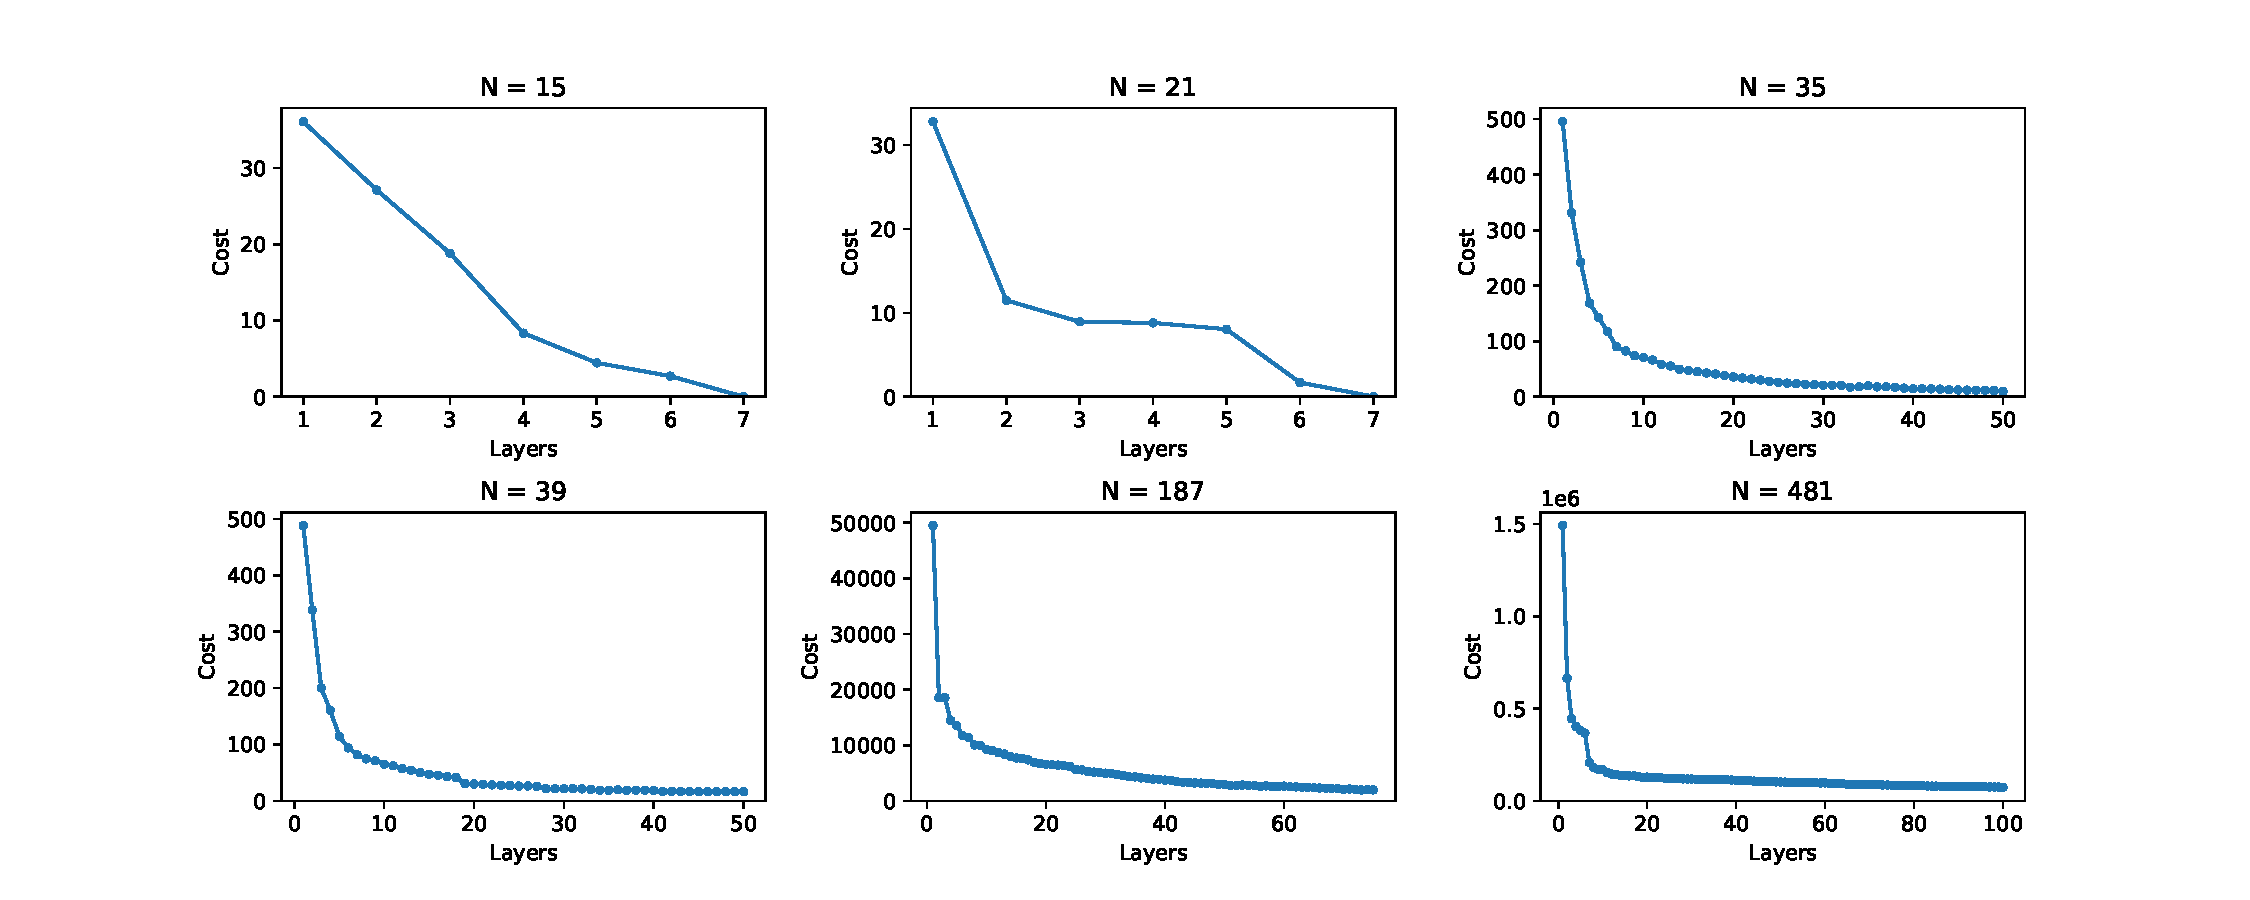
\includegraphics[width=1\textwidth]{cost_layers.pdf}
        \caption{Cost vs layers for different numbers. Notice the monotonically cost decreasing
        as the number of layers increases. Optimizer: L-BFGS-B.}
        \label{fig:cost_layers}
    \end{figure}
    
    \item Now angles evolve almost monotonically: $\gamma$ increases and $\beta$ decreases, similarly
    to adiabatic protocols.~(Fig.~\ref{fig:angle_evolution}). I am not sure if the evolution
    should be even smoother.
    \begin{figure}[h]
        \centering
        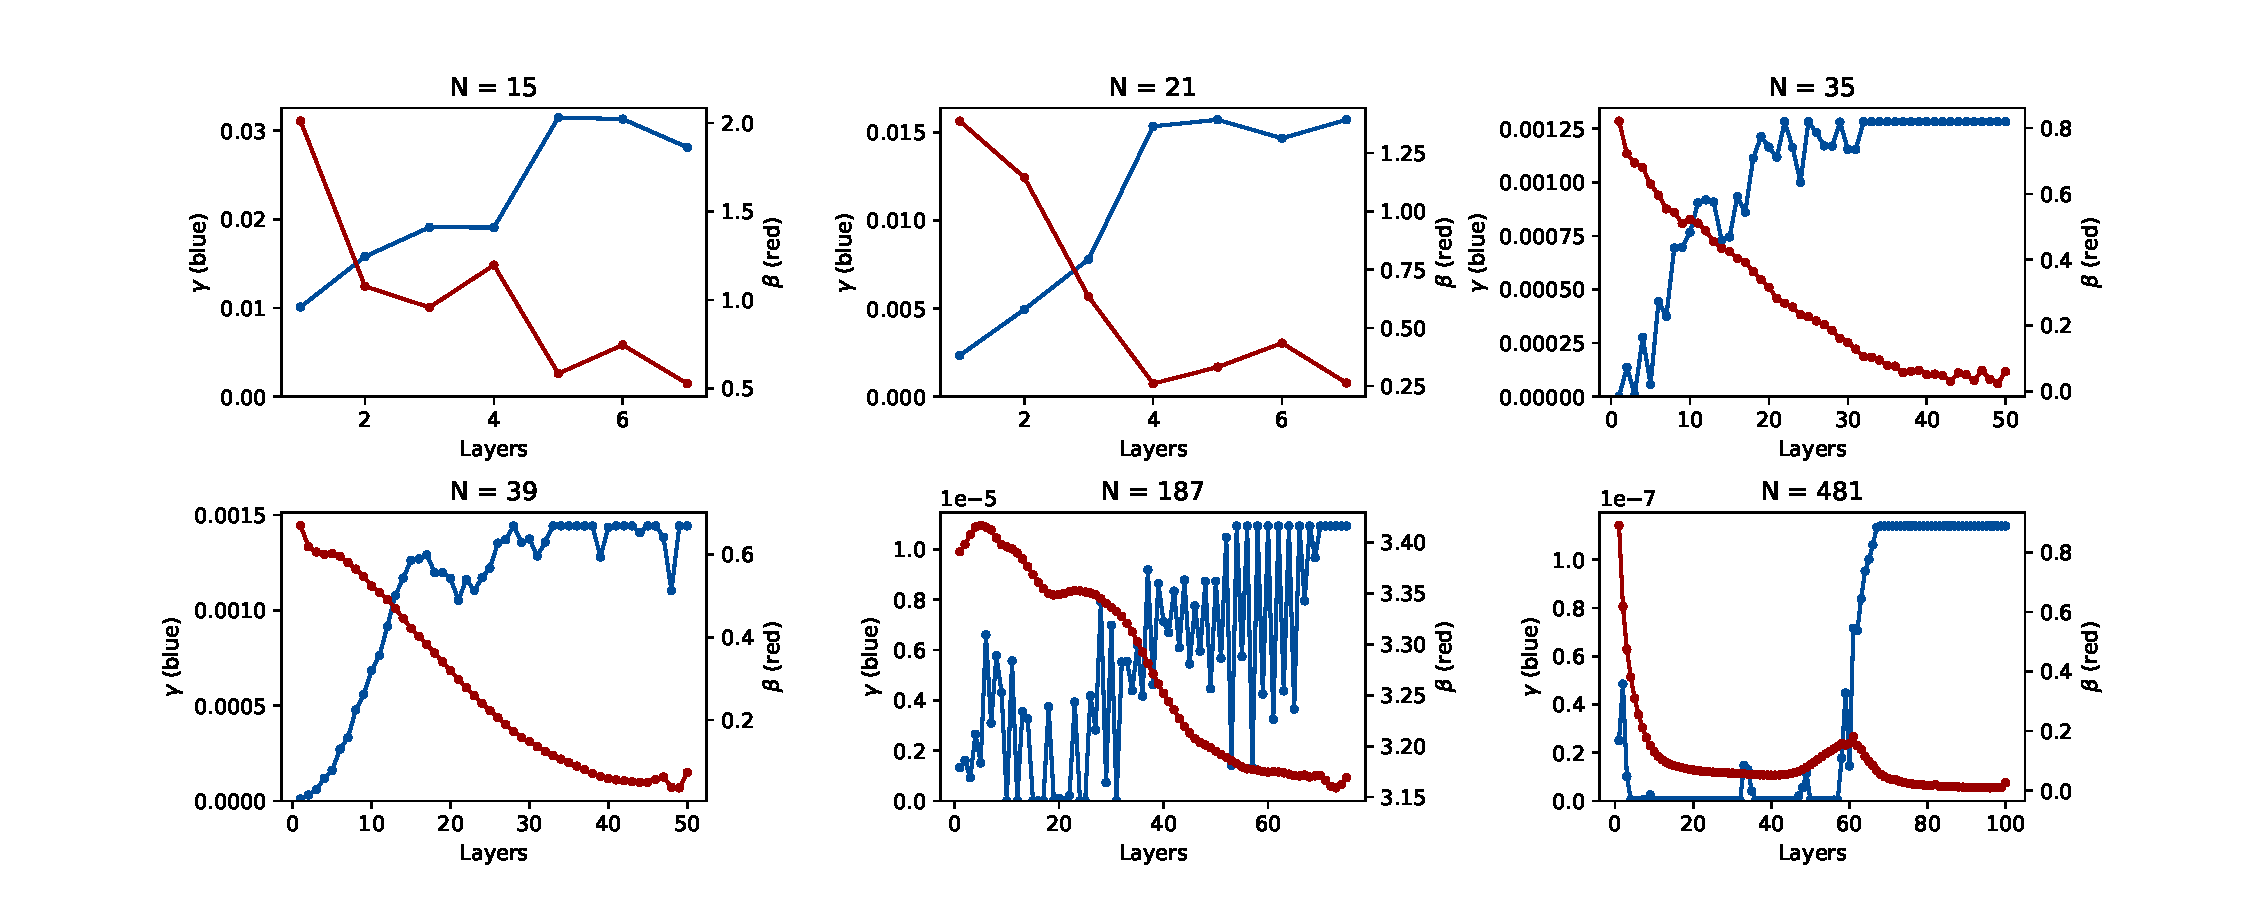
\includegraphics[width=1\textwidth]{angle_evolution.pdf}
        \caption{Angle evolutions for different $N$. Similarly to adiabatic protocols,
        the transverse field evolves from maximum to zero, while the interaction field
        does the opposite. Optimizer: L-BFGS-B.}
        \label{fig:angle_evolution}
    \end{figure}

    \item The probability vs energies plots look better than before~(Fig.~\ref{fig:prob_eigenstates}).
    \begin{figure}[h]
        \centering
        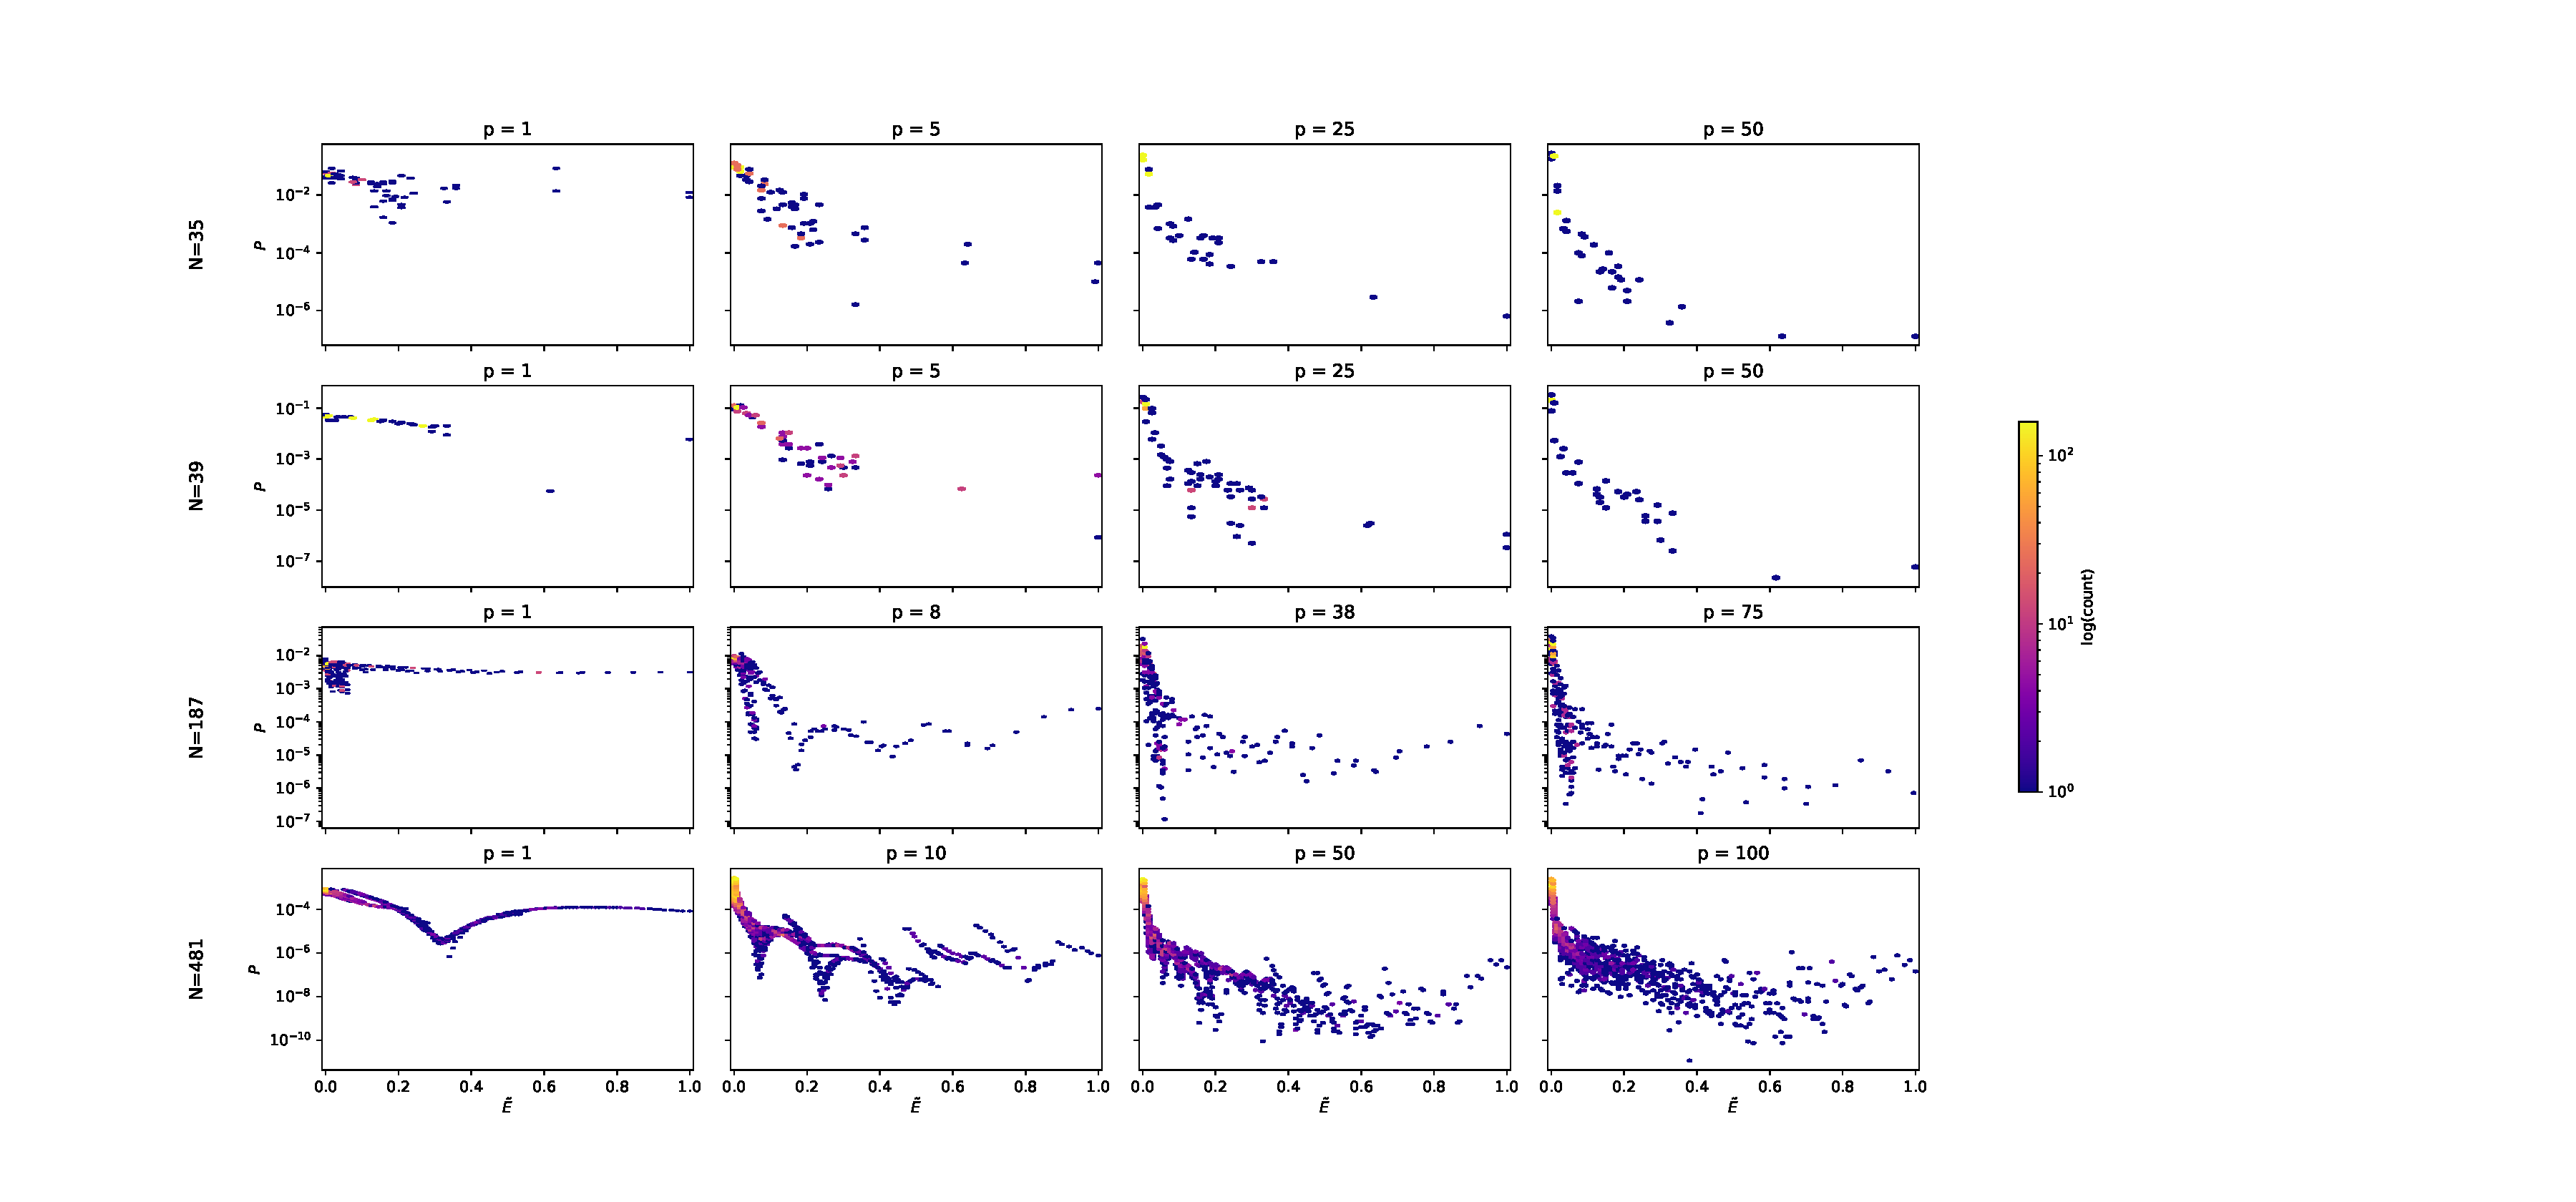
\includegraphics[width=1\textwidth]{prob_eigenstates.pdf}
        \caption{Density plots (probability vs rescaled energy) for some number of layers.
         Optimizer: L-BFGS-B.}
        \label{fig:prob_eigenstates}
    \end{figure}
\end{itemize}

\noindent Additionally, I found interesting to plot cost vs solution's fidelity for the different
target biprimes~(Fig.~\ref{fig:cost_fidelity}). 
\begin{figure}[h]
    \centering
    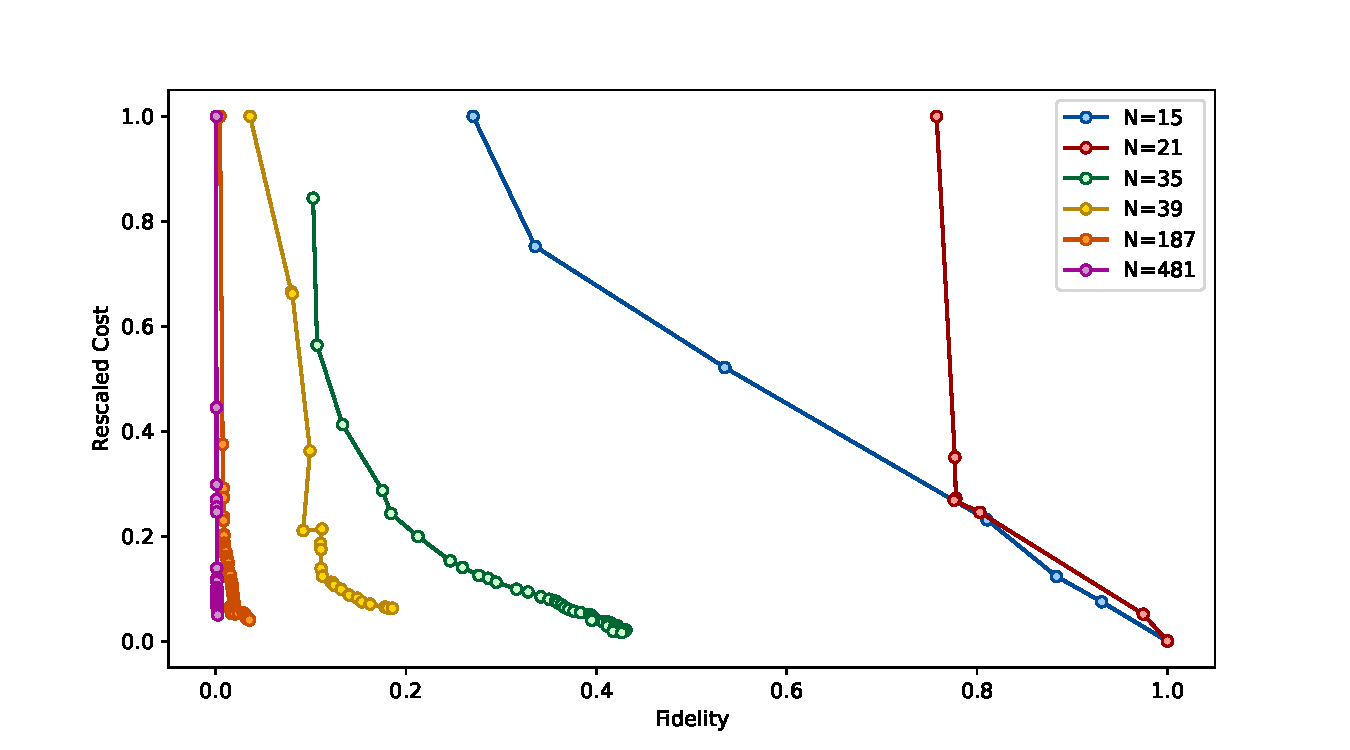
\includegraphics[width=1\textwidth]{cost_fidelity.pdf}
    \caption{Correlations between cost and fidelity with respect to the solution. Fidelity
    improvement becomes much more expensive for bigger problems. For $N=481$, the initial reduction
    of the cost function leads to only a tiny improvement in terms of fidelity. Optimizer: L-BFGS-B.}
    \label{fig:cost_fidelity}
\end{figure}

\subsection{Comparing with an unbounded method (BFGS)}
I have been wondering why in the past we got perfect solutions even we didn't restrict
the angles as explained at the beginning of this document. For example, BFGS is an unbounded
optimizer, we cannot restrict the angles in the desired intervals.
In fact, looking at~Fig.~\ref{fig:unbounded_pops}, we observe better results for BFGS than
for the bounded L-BFGS-B.

\begin{figure}[h]
    \centering
    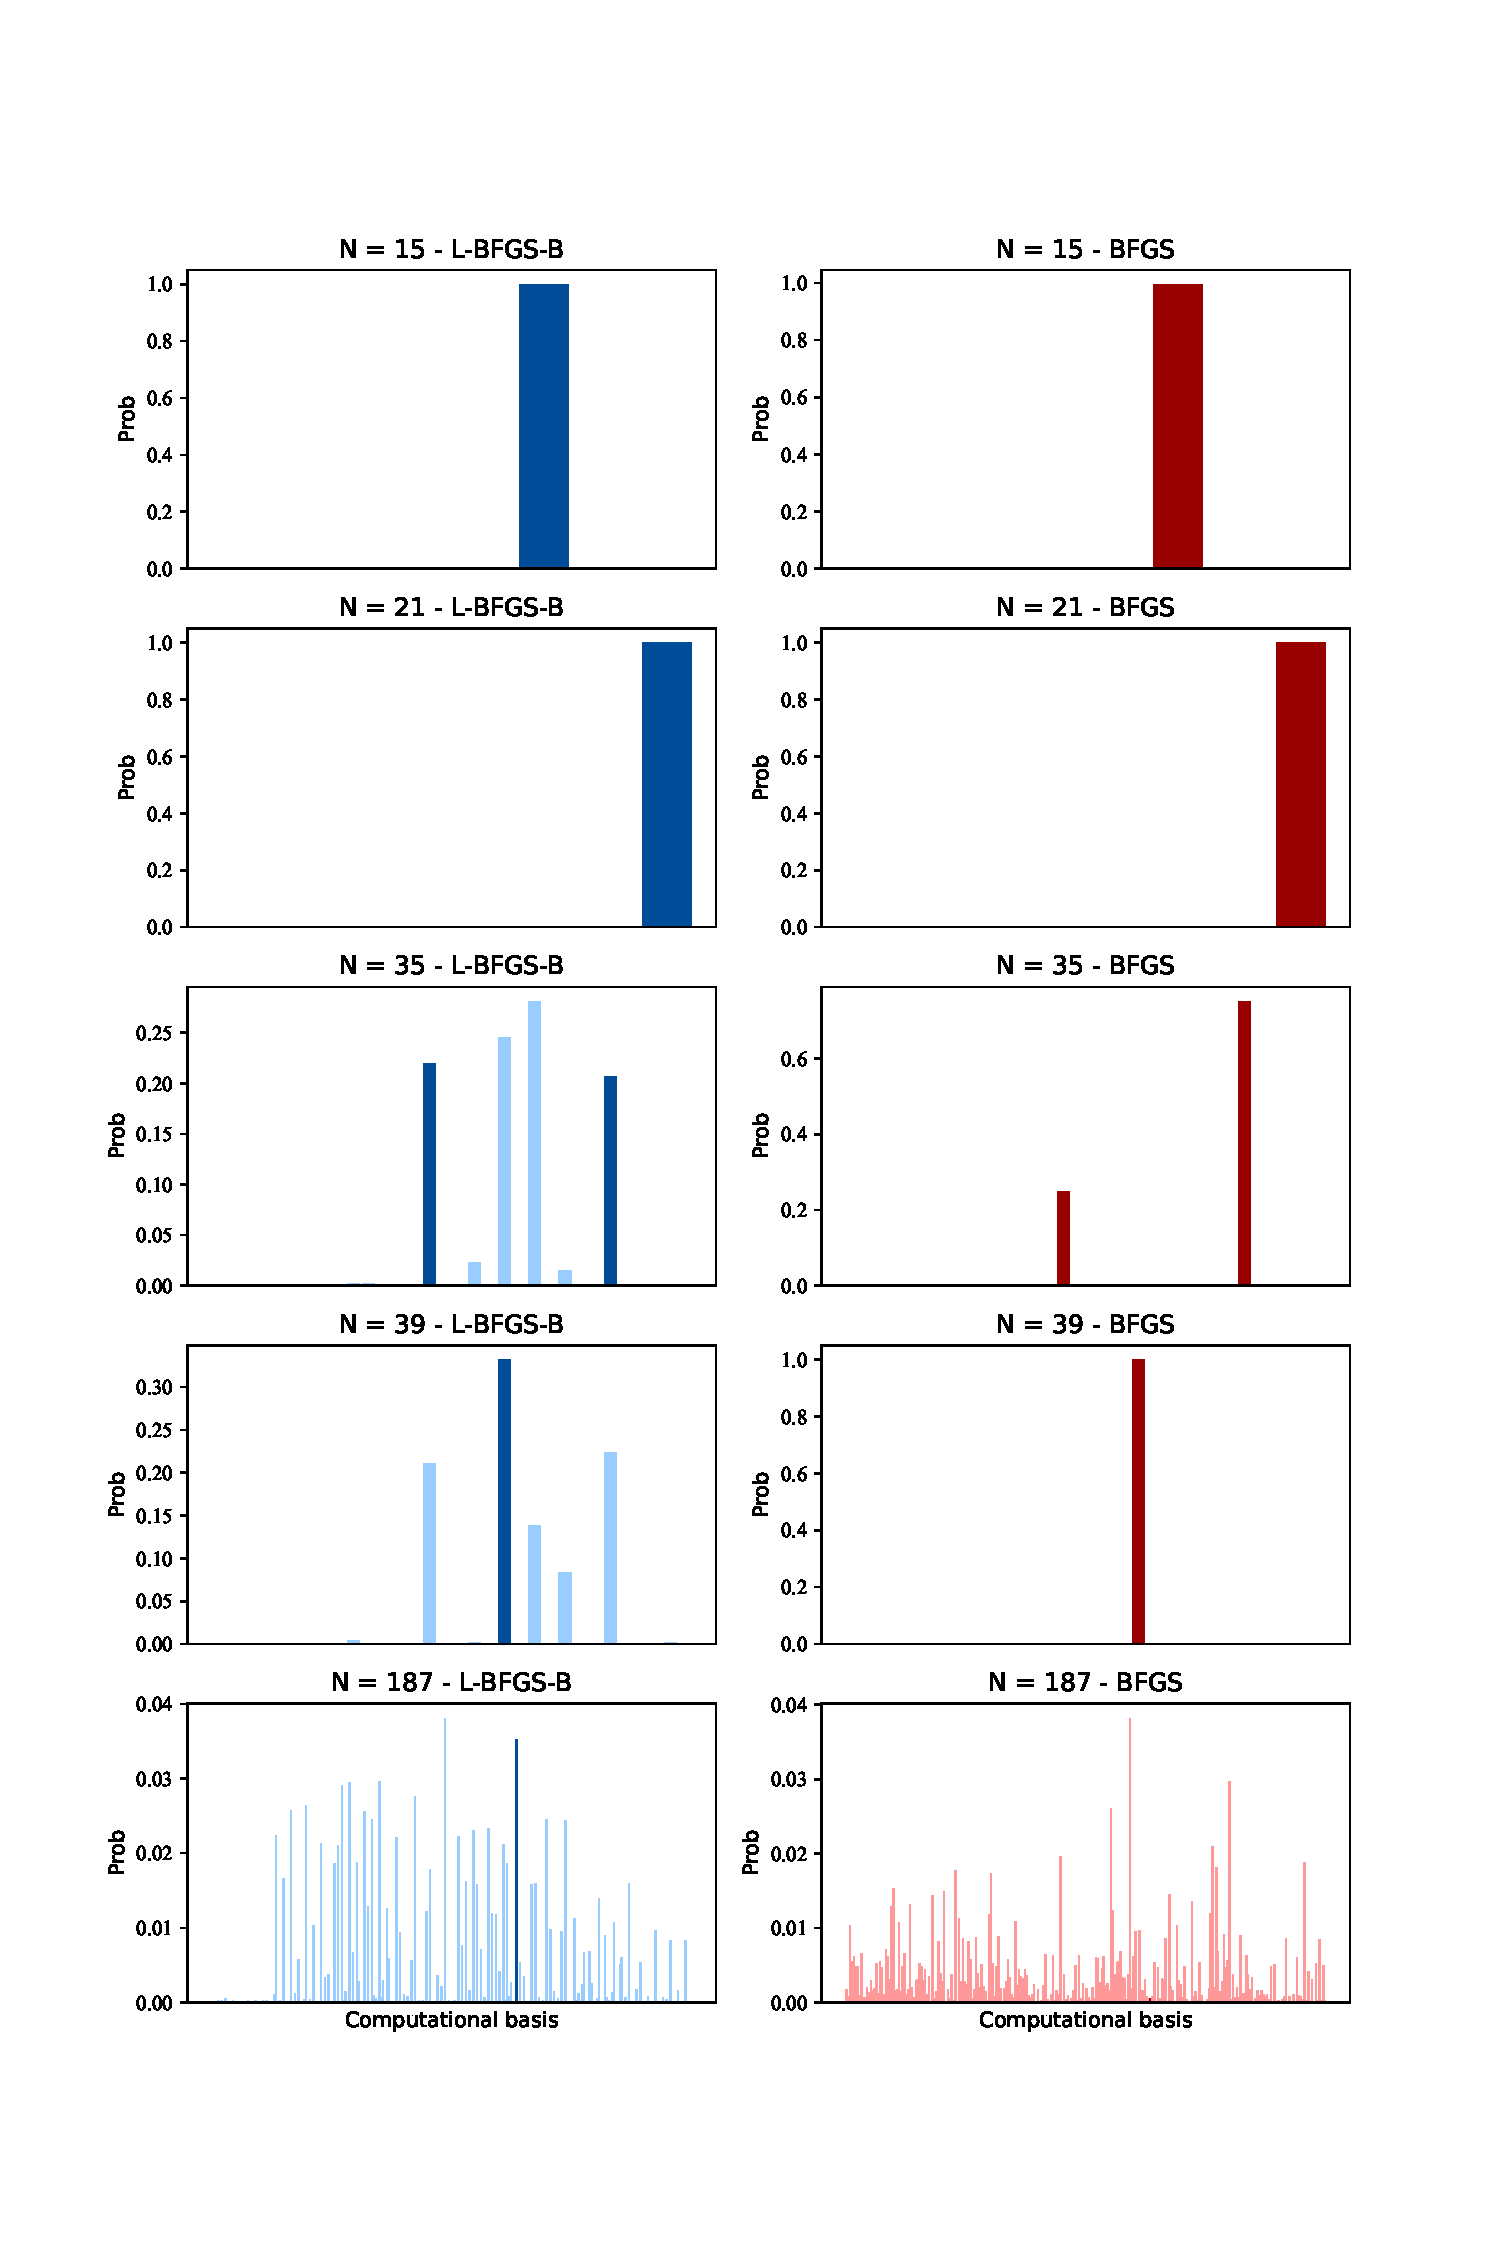
\includegraphics[width=0.8\textwidth]{unbounded_populations.pdf}
    \caption{Populations at the end of our algorithm. In the left,
    L-BFGS-B (bounded) optimizer has been used. In the right, BFGS (unbounded) has been used.}
    \label{fig:unbounded_pops}
\end{figure}

In Fig.~\ref{fig:unbounded_cost_evolution}, the evolution of the cost in our protocol for both optimizers is shown.
It is interesting to see that, in some cases, even not being monotonically decreasing, BFGS
finds the best solution much before than L-BFGS-B. The angles $\gamma$ and $\beta$ don't
behave as in the adiabatic protocol anymore, but it seems like it finds shorcuts to adiabaticity.
It is not a general behavior, and it is quite dependent on initial conditions, but
I frequently found it for small numbers.

\textbf{I think that's the explanation why we didn't notice that our old general algorithm was not adequate.}

\begin{figure}[h]
    \centering
    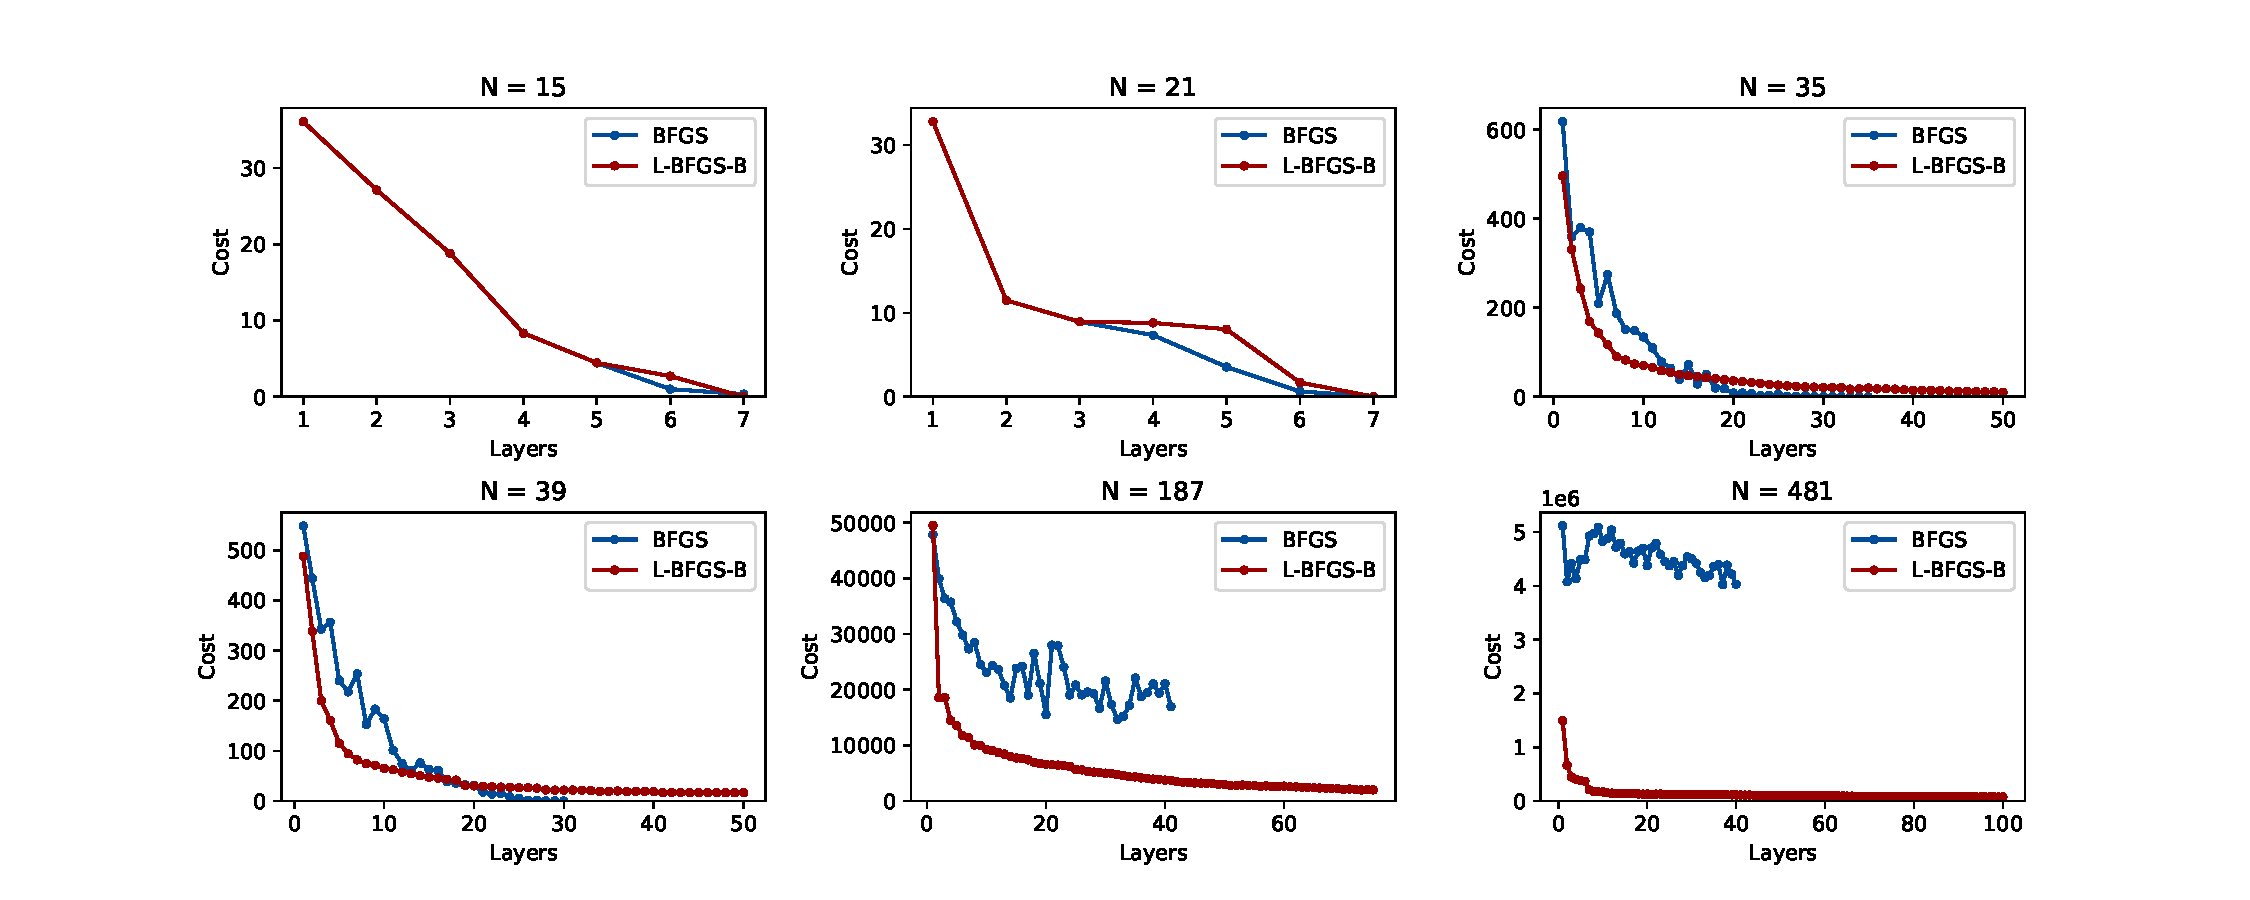
\includegraphics[width=1\textwidth]{unbounded_cost_evolution.pdf}
    \caption{Cost evolution with number of layers for BFGS (unbounded) and
    L-BFGS-B (bounded).}
    \label{fig:unbounded_cost_evolution}
\end{figure}

\end{document}